\documentclass[uplatex]{article}
\usepackage{luatexja}
\usepackage{tikz}
\usepackage{amsmath}
\usepackage{geometry}
\usepackage{tcolorbox} % 囲み枠用
\tcbuselibrary{skins, breakable}
\geometry{margin=2.5cm}

% 囲み定義用のスタイル:塗りなし、枠あり
\tcbset{
  mybox/.style={
    enhanced,
    colback=white,   % 背景を白(塗りなし)
    colframe=black,  % 枠線の色
    boxrule=0.8pt,
    arc=2mm,
    left=6pt,
    right=6pt,
    top=6pt,
    bottom=6pt,
    breakable
  }
}

\title{ベクトルの導入教材}
\author{}
\date{}

\begin{document}
\maketitle

\section*{1. ベクトルの加法}

\begin{tcolorbox}[title=定義:ベクトルの加法, mybox]
2つのベクトル $\vec{a}$, $\vec{b}$ の和 $\vec{a} + \vec{b}$ は、$\vec{a}$ の終点に $\vec{b}$ の始点を合わせ、始点から終点に向かうベクトルとして定義される。
\end{tcolorbox}

\begin{center}
\begin{tikzpicture}[scale=1.2]
  \draw[->, thick] (0,0) -- (2,1) node[midway, above] {$\vec{a}$};
  \draw[->, thick] (2,1) -- (4,3) node[midway, right] {$\vec{b}$};
  \draw[->, thick, dashed] (0,0) -- (4,3) node[midway, below left] {$\vec{a} + \vec{b}$};
  \fill (0,0) circle (2pt) node[below left] {O};
\end{tikzpicture}
\end{center}

\vspace{1em}

\section*{2. ベクトルの減法}

\begin{tcolorbox}[title=定義:ベクトルの減法, mybox]
2つの点 $A$, $B$ に対して、点 $A$ から点 $B$ へ向かうベクトルを $\vec{AB}$ とするとき、$\vec{a} - \vec{b}$ は、ベクトル $\vec{b}$ の終点からベクトル $\vec{a}$ の終点へ向かうベクトルと定義される。
\end{tcolorbox}

\begin{center}
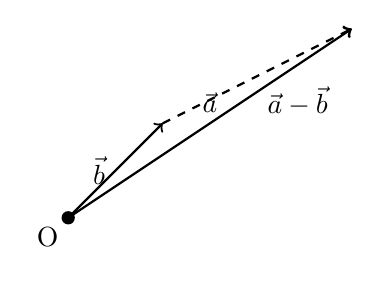
\begin{tikzpicture}[scale=1.2]
  \coordinate (O) at (0,0);
  \coordinate (A) at (3,2);
  \coordinate (B) at (1,1);

  \draw[->, thick] (O) -- (A) node[midway, above] {$\vec{a}$};
  \draw[->, thick] (O) -- (B) node[midway, left] {$\vec{b}$};
  \draw[->, thick, dashed] (B) -- (A) node[midway, below right] {$\vec{a} - \vec{b}$};

  \fill (O) circle (2pt) node[below left] {O};
\end{tikzpicture}
\end{center}

\vspace{1em}

\section*{3. 逆ベクトル}

\begin{tcolorbox}[title=定義:逆ベクトル, mybox]
ベクトル $\vec{a}$ に対して、向きが逆で大きさが等しいベクトルを $\vec{a}$ の逆ベクトルといい、$-\vec{a}$ と表す。$\vec{a} + (-\vec{a}) = \vec{0}$ が成り立つ。
\end{tcolorbox}

\begin{center}
\begin{tikzpicture}[scale=1.2]
  \draw[->, thick] (0,0) -- (2,1) node[midway, above] {$\vec{a}$};
  \draw[->, thick] (0,0) -- (-2,-1) node[midway, below] {$-\vec{a}$};
  \fill (0,0) circle (2pt) node[below left] {O};
\end{tikzpicture}
\end{center}

\end{document}
